\documentclass[a4paper,12pt]{article}
\usepackage[T1]{fontenc}
\usepackage[dvipsnames]{xcolor}
\usepackage[utf8x]{inputenc}
\usepackage[russian]{babel}
\usepackage{pdflscape}
\usepackage{fancyvrb}
\usepackage{geometry}
\usepackage{indentfirst}
\usepackage{wrapfig}
\usepackage{placeins}
\usepackage{graphicx}
 \geometry{
 a4paper,
 total={210mm,297mm},
 left=10mm,
 right=20mm,
 top=10mm,
 bottom=15mm,
 }

\usepackage{listings}
\lstset{basicstyle=\ttfamily,
  showstringspaces=false,
  commentstyle=\color{OliveGreen},
  keywordstyle=\color{MidnightBlue},
  extendedchars=\true,
  inputencoding=utf8x,
  breaklines=true,
  basicstyle=\ttfamily\footnotesize
}

\RecustomVerbatimCommand{\VerbatimInput}{VerbatimInput}%
{fontsize=\scriptsize,
 %
 %frame=lines,  % top and bottom rule only
 %framesep=2em, % separation between frame and text
 rulecolor=\color{Gray},
 %
 %label=\fbox{\color{Black}text2},
 %labelposition=topline,
}
\begin{document}

\begin{titlepage}
  \begin{center}
    \large
    Міністерство освіти і науки України
    
    Національний технічний університет України

    \textit{“Київський політехнічний інститут”}
    
    Фізико-технічний інститут
    \vspace{5cm}

    \textsc{Лабораторна робота №1}\\[5mm]
    
    {\LARGE Експериментальна оцінка ентропії на символ джерела\\
	відкритого тексту. Криптоаналіз шифру Віженера}\\
  \bigskip
    
    
\end{center}
\vspace{3cm}
\hfill
\begin{minipage}{0.3\textwidth}
\large
  Виконав:\\
  \textit{Грубіян Є.О.}\\
  Прийняв:\\
  \textit{Яковлєв С.В.}\\ % aka Euler
  
\end{minipage}
\bigskip

\vfill
\vfill
\vfill
\begin{center}
  Київ 2015 р.
\end{center}

\end{titlepage}
\section*{Обчислення \( H_1 \) }
{\large Скрипт обчислення \( H_1 \) та частотного аналізу для твору 'Ідіот' Достоєвського:}\\
\lstinputlisting[language=python]{freq.py}
\newpage
{\large Результати для тексту з пробілами: }
\VerbatimInput{freq2.txt}

{\large Результати для тексту без пробілів: }
\VerbatimInput{freq.txt}

\section*{Обчислення \( H_2 \) }
{\large Скрипт обчислення \( H_2 \) та частотного аналізу біграм для твору 'Ідіот' Достоєвського}\\
\lstinputlisting[language=python]{freq2.py}
\begin{landscape}
{\large Результати для тексту з пробілами: }
\VerbatimInput{bigram2.txt}
\end{landscape}
\begin{landscape}
{\large Резульати для тексту без пробілів: }
\VerbatimInput{bigram.txt}
\end{landscape}
\newpage
\section*{Визначення умовних ентропій \( H^{(10)}, H^{(20)}, H^{(30)} \) }
\begin{figure}[h]
  \begin{center}
    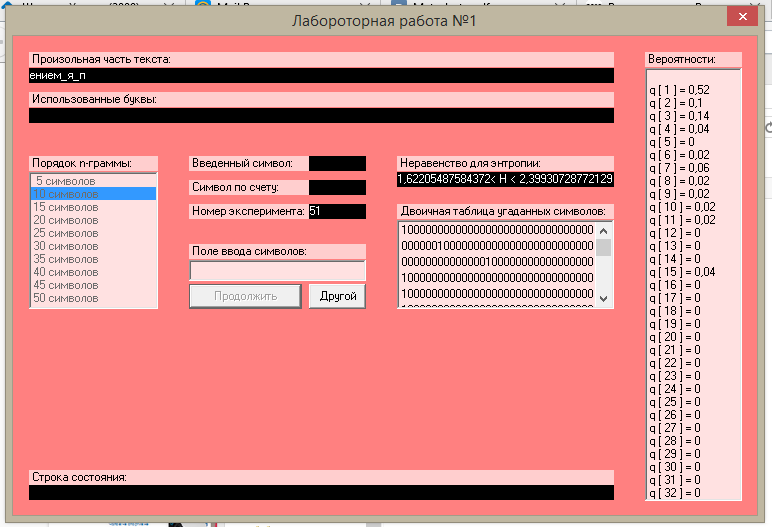
\includegraphics[width=0.97\textwidth]{1.png}
  \end{center}
  %\caption{H(10)}
\end{figure}
%\newpage
\begin{figure}[h]
  \begin{center}
    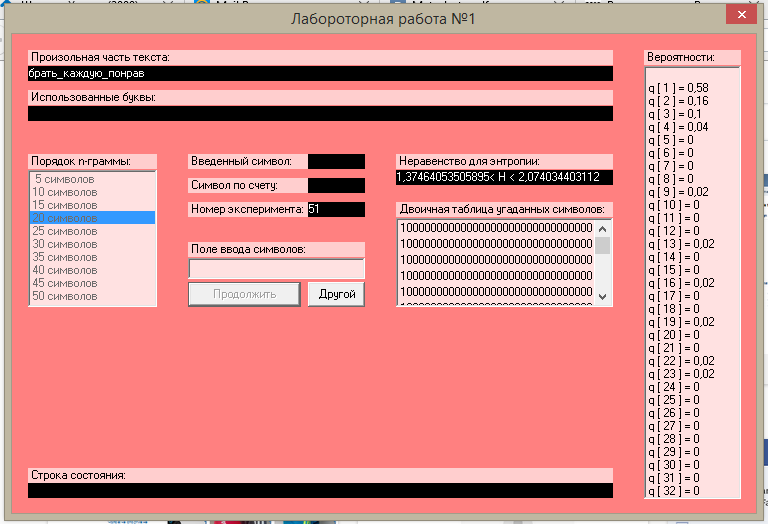
\includegraphics[width=0.97\textwidth]{2.png}
  \end{center}
  %\caption{H(20)}
\end{figure}
%\newpage
\begin{figure}[h]
  \begin{center}
    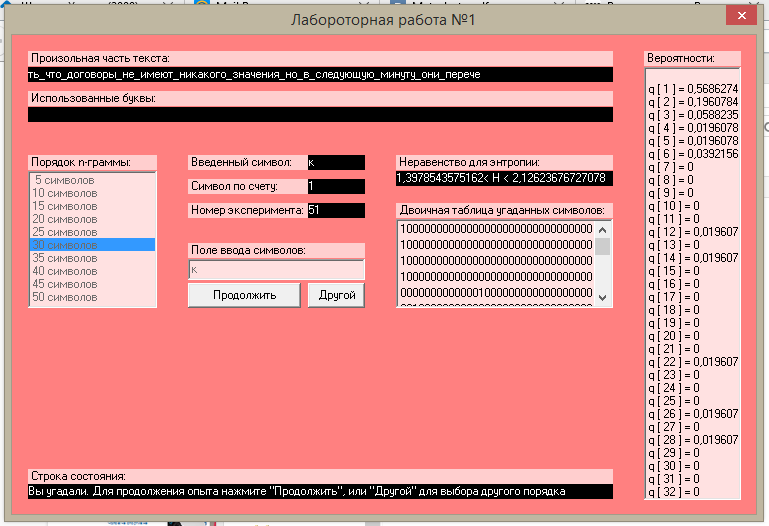
\includegraphics[width=0.97\textwidth]{3.png}
  \end{center}
  %\caption{H(30)}
\end{figure}
\FloatBarrier
\newpage
\section*{Криптоаналіз шифру Віженера}
{\large Скрипт криптоаналізу шифру Віженера:}
\lstinputlisting[language=python]{vigenere.py}
{\large Результат криптоаналізу шифру Віженера:}
\VerbatimInput{tmp.txt}
\section*{Висновок}
В лабораторній роботі було зроблено частотний аналіз різних текстів та визначено ентропії \( H_1 \) та \( H_2 \), а також проведено криптоаналіз шифру Віженера та встановлено ключ яким зашифровувався текст.
\end{document}
